<!-- 
=========================================
TEASER FIGURE PLACEHOLDER
(For CVPR format, place this at the top of the first page or immediately after \maketitle)
=========================================
\begin{figure*}[t]
  \centering
  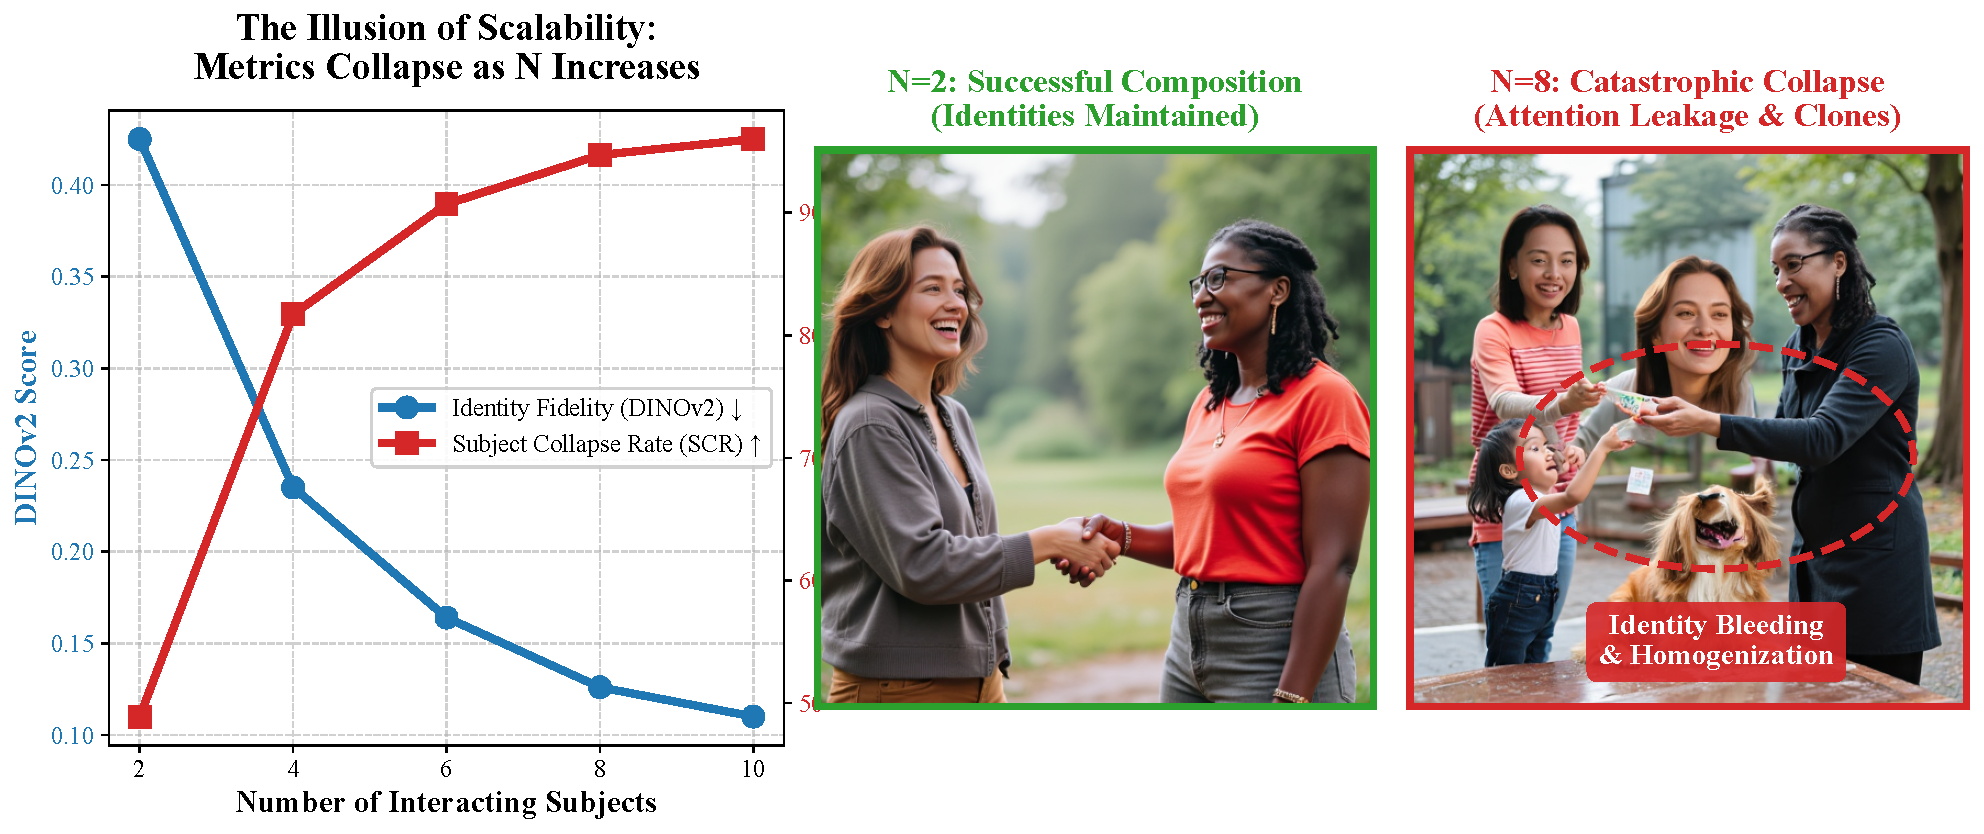
\includegraphics[width=\textwidth]{figures/teaser.pdf}
  \caption{\textbf{Catastrophic Identity Collapse in Multi-Subject Personalization.} 
  (Left) State-of-the-art models like MOSAIC~\cite{mosaic2024} perform well when composing 2 subjects. 
  (Right) When evaluated on our proposed stress-test benchmark with 8 interacting subjects, models suffer from severe identity blending, feature homogenization, and attention leakage. 
  Our novel Subject Collapse Rate (SCR) metric effectively captures this degradation, revealing a critical gap in current generative systems.}
  \label{fig:teaser}
\end{figure*}
-->

## Abstract

Subject-driven text-to-image diffusion models [1, 2] have achieved remarkable success in preserving single identities, yet their ability to compose multiple interacting subjects remains largely unexplored and highly challenging. Existing evaluation protocols typically rely on global CLIP metrics [3], which are insensitive to local identity collapse and fail to capture the severity of multi-subject entanglement. In this paper, we introduce a comprehensive stress-test benchmark designed to evaluate multi-subject personalization under varying degrees of complexity, ranging from 2 to 10 interacting identities. To accurately measure identity preservation, we shift the evaluation paradigm from CLIP-based similarity to DINOv2 [4] feature matching, and propose a novel metric, Subject Collapse Rate (SCR), to explicitly quantify the proportion of identity loss in generated scenes. We conduct an extensive evaluation of recent state-of-the-art models (MOSAIC [5], XVerse [6], PSR [7]) under our benchmark. Our quantitative and qualitative results reveal a catastrophic failure in current models: as the number of subjects increases, the SCR approaches 100%, indicating complete identity confusion and attention leakage. Furthermore, we uncover a critical trade-off where models sacrifice fine-grained identity fidelity (DINOv2) to maintain macro-level text-image alignment (CLIP-T). Our benchmark and metrics highlight a significant gap between semantic and physical disentanglement, providing a rigorous foundation for future research in multi-subject generative systems.
